\documentclass{article} % For LaTeX2e
% We will use NIPS submission format
\usepackage{nips13submit_e,times}
% for hyperlinks
%\usepackage{hyperref}
\usepackage{url}
% For figures
\usepackage{graphicx} 
\usepackage{subfigure} 
% math packages
\usepackage{amsmath}
\usepackage{amsfonts}
\usepackage{amsopn}
\usepackage{ifthen}
\usepackage{natbib}
\usepackage{color}
\usepackage{float}
\usepackage{placeins}
\usepackage{geometry}
\usepackage{listings}

\title{Project-II by Group Istanbul}

\author{
Johan Droz\\
EPFL \\
\texttt{johan.droz@epfl.ch} \And
Arseniy Zaostrovnykh\\
EPFL \\
\texttt{arseniy.zaostrovnykh@epfl.ch}
}

% The \author macro works with any number of authors. There are two commands
% used to separate the names and addresses of multiple authors: \And and \AND.
%
% Using \And between authors leaves it to \LaTeX{} to determine where to break
% the lines. Using \AND forces a linebreak at that point. So, if \LaTeX{}
% puts 3 of 4 authors names on the first line, and the last on the second
% line, try using \AND instead of \And before the third author name.

\nipsfinalcopy 

\newcommand{\todo}[1]{}
\renewcommand{\todo}[1]{{\color{red} TODO: {#1}}}

\begin{document}

\maketitle

\begin{abstract}
In this report we describe our results for the second project of the 2015 PCML class.
Our goal is to design a system that, given an image, is able to recognize three kinds of object in it.
We tried to improve the accuracy of the system by experimenting with different methods.

\end{abstract}

\section{Data Description}

The system we have to design has to be able to classify images based on what object they contain. 
There are 4 classes: the image can contain an airplane, a car, a horse or neither of them.

A training set containing either color or grayscale images of size 231x231 is given. It contains 6000 images, each associated with a label and two sets of features: the Histogram of Oriented Gradients (HOG) and the OverFeat ImageNet CNN Features.

For acceleration of the experiments, we considered the ways to reduce the number of features. 

One ways is to scale down the input images. However, this affectts only the HOG features, as CNN represents the neural network weights and does not depend on the number of pixels in the image.

The CNN feature array seems very sparse. However an investigation shown that each feature(except for the last one) is nonzero for at least 20 images in the train set.

Other way is to find correlations in that matrix. no way: number of features ~36000, number of datapoints 6000 -> matrix rank is going to be <= 6000 => there are a lot of linear combinations of the columns.

Note: move from small-pics to the originals require a complete recalibration of SVM meta-parameters

Note: hard-negative mining

Note: the best-optimized SVM(HOG) gives 0.1734 test BER and 0.0554 train BER on 3-fold cross validation.

\paragraph{HOG feature} HOG is widely use in computer vision. 
The basic idea is that the shape and appearance of an object is often well characterized by the distribution of local intensity gradients or edge directions \cite{hog}.
Figure \ref{fig:image_car} and \ref{fig:hog} shows respectively an image form the training set and a visualization of its HOG feature.
And in fact, the shape of the car is recognizable in the HOG visualization.

\paragraph{CNN features} Features extracted from the OverFeat convolutional neural network (CNN).

\begin{figure}[!t]
	\centering
	\subfigure[Training image]{\label{fig:image_car}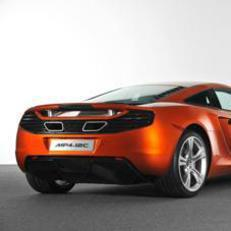
\includegraphics[width=0.4\textwidth]{figures/train00003.jpg}}
	\hspace{10pt}
	\subfigure[HOG feature]{\label{fig:hog}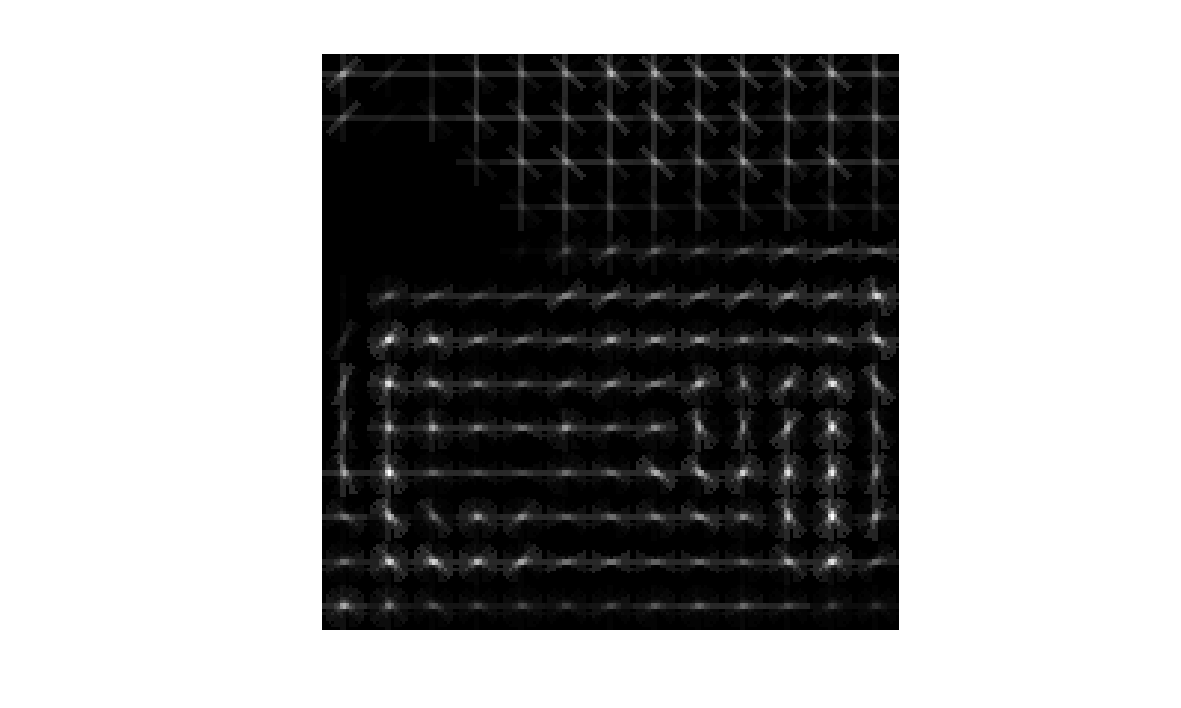
\includegraphics[width=0.4\textwidth]{figures/hog.pdf}}
	\caption{Visualization of the HOG feature}
\end{figure}

The testing set contains only the HOG and CNN features and not the images from which those feature are extracted.
As a consequence we should focus on optimizing the classification based on these two set of features, and not trying to extract different one.
The testing set contains 11'453 samples and we have to submit two predictions: a binary prediction, that is whether the image contains either a car, a plane or a horse, or neither of them and a multiclass 
prediction, where we predict the object present in the image.

\paragraph{Training data}

I do not think that a horse, a car and an airplane share any common structure, so it its reasonable to do binary prediction based on the multiclass prediction. Simply:
y = (y ~= 4)  -- if classifier have not found any of these three, answer no.

Each class should be detected separately, of course:

\begin{lstlisting}

if (y_{horse} == 1) y = 1
else if (y_{car} == 1) y = 2
else if (y_{airplane} == 1) y = 3
else y = 4
end
\end{lstlisting}

We should think how do we handle disputed cases (e.g. $y_{horse}$ == 1 and $y_{car} == 1$). we may train 3 additional classifiers for each of those (if we get enough cases for it).

\section{Data visualization and basic exploratory data analysis}


\subsection{Performance measures}

\section{Predict test data}

%\begin{figure}[!t]
%	\centering
%	\subfigure[Scatter plot of one input variable vs output]{\label{fig:scatter}\includegraphics[width=0.55\textwidth]{figures/X58vsY.pdf}}
%	\subfigure[Histogram of $\boldmath{y\_train}$]{\label{fig:histY}\includegraphics[width=0.4\textwidth]{figures/histY.pdf}}
%	\caption{Data analysis}
%\end{figure}



%\begin{figure}[!t]
%	\center
%	\includegraphics[width=0.8\textwidth]{figures/ridgeRegLoss.pdf}
%	\caption{Plot of the test and training error for ridge regression}
%	\label{fig:ridgeRegError}
%\end{figure}


\section{Summary}
\bibliographystyle{plain}
\bibliography{References.bib}

\end{document}
